\documentclass{article}
% setup page
\usepackage[utf8]{inputenc}
\usepackage{fancyhdr}
\usepackage[a4paper, top=2.2cm, left=1.5cm, right=1.5cm, bottom=1.75cm]{geometry}
\usepackage{titling}

\usepackage{todonotes}
\usepackage{amsmath}
\usepackage{graphicx,wrapfig}
\usepackage[font=small,labelfont=bf]{caption}

\usepackage[backend=biber]{biblatex}
\addbibresource{papers.bib}

% setup info
\title{IR Project 1: Report}
\author{Tobias Veto, Philip Junker, Marc Fischer}

% setup header/footer
\pagestyle{fancy}
\fancyhf{}
\rhead{\theauthor}
\lhead{\thetitle}
\rfoot{Page \thepage}


\begin{document}

\section*{Introduction}
For the implementations of the naive Bayes, logistic regression and SVM we stayed close to the code shown in the lecture. Thus the implementations of the algorithms were straightforward while optimization and data pre-processing were challenging. Most of our effort went into the data pruning.

In our team one person each focused on one classifier. While we shared insights and the code that we use for the reader, this might account for inconsistencies in the code and different tone in the chapters of this report.

\vspace{-2mm}
\section*{Data transformation and pruning}
A big part of our implementation was data preprocessing. We read the tokens from the documents (with the tinyIR library), removed tokens not consisting of letters, stemmed the word and removed stopwords. \cite{joachims_text_1998,ozgur_text_2005} both list this as the standard approach to pre-processing in document classification. From the resulting corpus of documents we remove those that occured in less then \texttt{minOccurrence} and those that are found in more than $\text{\texttt{maxOccurrenceRate}} \cdot \text{\texttt{nrDocuments}}$, where $\text{\texttt{maxOccurrenceRate}} \in (0, 1]$.
The resulting dictionary of words is used to represent each document as a bag-of-words vector. For the weights within the vector we used boolean weights (1 if the word occurs in the document, else 0), tf-idf weights (inspired by \cite{ozgur_text_2005}) and the word frequency. The latter generally lead to the best results.
We also discovered  that words extracted from the title of the document contain a high amount of information and lend themselves especially to predicting country codes. The words from the titles were processed like the words from the content.

Because the initial documents have more influence in online algorithms such as our SVM and Logistic Regression, we tried accessing the documents of the training set in random order. The hope was to spread the influence of documents more evenly across the corpus. However this did not lead to significant improvements.

Predicting the industry codes turned out to be very difficult : There were more possible industry codes, and some of them were very rarely assigned.  In addition, we observed that around half of the documents did not have any industry code assigned. For Logistic Regression and Naive Bayes, we therefore chose to never assign any industry code. This lead to better results as the precision remained unaffected.

\vspace{-2mm}
\section*{Naive Bayes}

\begin{wrapfigure}{r}{6cm}
    \centering
    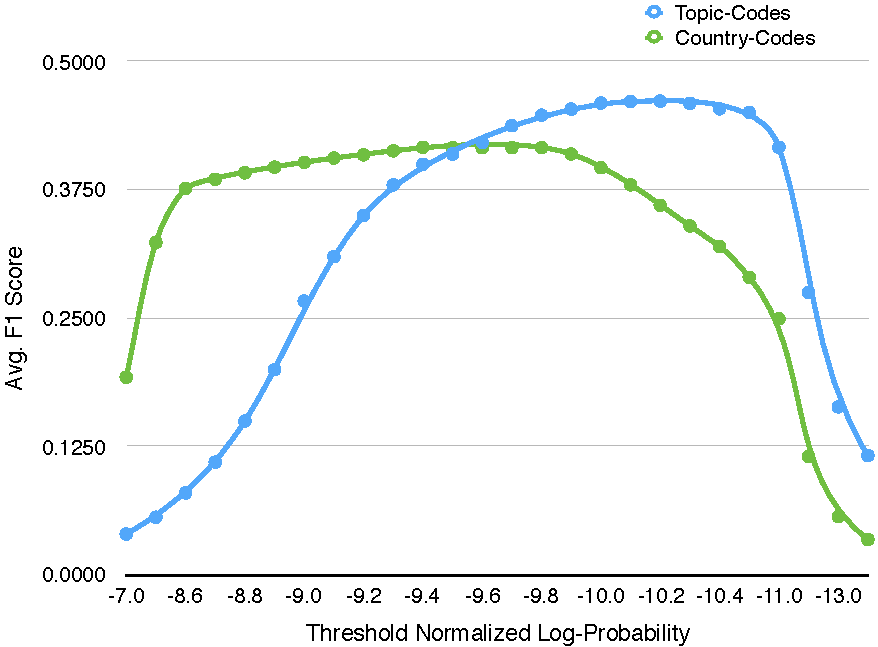
\includegraphics[width=6cm]{graphics/BayesF1ScoreTopicCountry.pdf}
    \caption{This figure shows the average F1-Score of topic- and country-codes using different thresholds for the normalized log-probability.}
    \label{fig_bayesThreshold}
\end{wrapfigure}

We used the formulas for Naive Bayes as shown in the lecture. For each code we calculated the probability $P(word | code)$ for every word in the reduced dictionary. We were then faced with the problem of finding cutoff values for probabilities that determine whether a code is assigned to a document or not.

For each of the three different code-types different cutoffs were evaluated. The advantage of this approach is the independence of the code-types and therefore the possibility of a country-code to be predicted although the probability for this code given a document is much lower than for all the topic-codes. The performance in form of F1-scores is plotted for both country- and topic-codes in figure \ref{fig_bayesThreshold}. As mentioned, no industry codes were predicted, and the document title was used instead of the document content to calculate probabilities for the country codes.

For the topic-codes the optimal threshold for the log-probabilities has been evaluated on the full training data to be $-10.2$ and for the country-codes $-9.4$. With these thresholds and the above mentioned approach of only considering article titles for training of country-codes and only considering content for training topic-codes we achieved an F1-Average score of $0.424$ on the validation set.

The training of the model needs constantly 1.3GB of RAM. The training of the topic-codes took around 160 minutes in total to train the topic-codes (80 minutes) and the country-codes (80 minutes). This was done on a laptop with an intel i7 (2.9GHz) with 8GB of RAM.


\vspace{-2mm}
\section*{Logistic Regression}
    Logistic regression was done as an online-algorithm with one-vs-all classifiers for each code. After pre-processing and pruning the data as described above, we had to select the \texttt{minOcccurence} and \texttt{maxOccurence} rate. We tried different values but saw that using \texttt{minOccurrence} = 20 and \texttt{maxOccurenceRate} = 1 lead to the best results.
    As in naive bayes, the three code types were treated independently :
    \begin{description}
    \item[Topic codes] For topic codes we tried to find a cutoff value such that the average number of codes assigned to a document remained the same in our prediction as in the test set. This was achieved with a "cutoffFinder" construct consisting of two priority queues. With this approach reached an F1-score of around 0.35 for topic codes.
    \item[Country codes] Again,  we had even better results when using the document title instead of the content. Also, the cutoff value was determined manually by trying different values : The cutoffFinder approach lead to worse results since the resulting codes were assigned unevenly across the documents. With our approach we reached a F1-score of around 0.44
    \item[Industry codes] As mentioned, we never predicted any Industry codes, because the negative impact on precision was too high.
    \end{description}

    Predicting the three label types separately and combining the predictions into one lead to an F1-score of around 0.36. One attempt at increasing the performance was to lower the learning rate, such that it would increase, for example, after 10 documents instead of 1. Also, different normalization techniques were tried, but none lead to significant improvement in performance. Our final algorithm required approximately 1.9 GB of memory and took around 12 minutes to compute an intel i7 laptop (2.9GHz) with 8GB of RAM.

\vspace{-2mm}
\section*{SVM}
The algorithm shown in the lecture is the well-known pegasos algorithm\cite{shalev-shwartz_pegasos:_2011,shalev-shwartz_pegasos:_????}. For the implementation we trained one SVM per category occurring in the training data in an all-vs-one approach.
Table~\ref{table:svmResults} shows the results of various approaches.
The data was preprocessed as introduced before with the use of homogeneous coordinates (bias term) and without. The listed papers suggest not using a bias with the normal formulation of the pegasos algorithm or to adjust it if doing so, as it undermines the convergences guarantee. As it only provided a very small change, we therefore did not include a bias. For the parameter $\lambda$ the optimal choice seems to be around $10^{-4} - 10^{5}$. Seems consistent when changing other parameter of the algorithm. Thus further tests were only run with those $\lambda$ values.

Reducing the dictionary size helped to reduce the run time of the algorithm and slightly increased the score. So the final version (bold) uses only tokens extracted from titles, but all of them.

Using the absolute count as weights of the bag-of-words vectors was equivalent to boolean weights when it comes to performance and slightly better than tf-idf weights.

\begin{table}[h]
\centering
\resizebox{\textwidth}{!}{
	\begin{tabular}{|l|l|l|l|r|r|r|r|r|r|}
	\hline
	$\lambda$ & \texttt{minOccurrence} & \texttt{maxOccurrenceRate} & Dictionary,Weights & Resulting \# Words & Run Time & Memory Consumption & Avg. Precession & Avg. Recall & Avg. F1-Score\\
	\hline
	1 & 1 & 0.2 & tokens, count-weights & 109995 & 123 min & 8 GB & 0.295 & 0.053 & 0.08\\ \hline
	1 & 3 & 0.2 & tokens, count-weights & 39249 & 28 min & 3.4 GB & 0.30 & 0.053 & 0.09\\ \hline
	0.1 & 3 & 0.2 & tokens, count-weights & 39249 & 28 min & 3.7 GB & 0.30 & 0.053 & 0.09\\ \hline
	0.01 & 3 & 0.2 & tokens, count-weights & 39249 & 19 min & 3.4 GB & 0.55 & 0.11 & 0.19\\ \hline
	0.001 & 3 & 0.2 & tokens, count-weights & 39249 & 15 min & 3.5 GB & 0.88 & 0.19 & 0.31\\ \hline
	0.0001 & 3 & 0.2 & tokens, count-weights & 39249 & 14 min & 3.4 GB & 0.92 & 0.20 & 0.33\\ \hline
	0.00001 & 3 & 0.2 & tokens, count-weights & 39249 & 14 min & 3.4GB & 0.92 & 0.20 & 0.33\\ \hline
	0.0001 & 10 & 0.2 & tokens, count-weights & 17521 & 7 min & 3 GB & 0.92 & 0.20 & 0.33\\ \hline
	0.0001 & 20 & 0.2 & tokens, count-weights & 11397 & 5 min & 2.9 GB & 0.92 & 0.20 & 0.33\\ \hline
	0.0001 & 20 & 1 & tokens, count-weights & 11420 & 5 min & 3.1 GB & 0.92 & 0.20 & 0.33\\ \hline
	\textbf{0.0001} & \textbf{0} & \textbf{1} & \textbf{titles, count-weights} & \textbf{22871} & \textbf{8 min} & \textbf{3.1 GB} & \textbf{0.94} & \textbf{0.21} & \textbf{0.34}\\ \hline
		0.0001 & 0 & 1 & titles, boolean weights & 22871 & 8 min & 3.1 GB & 0.94 & 0.21 & 0.34\\ \hline
	0.0001 & 0 & 1 & titles, tf-idf weights & 22871 & 8 min & 3.1 GB & 0.90 & 0.20 & 0.32\\ \hline

	\end{tabular}
}
\caption{Test Results for the SVM. All tests were done on a Machine with 32 GB ram and a high java heap size, thus java never deallocated memory. On another machine with less memory the memory consumption of the SVM code took only around 2 GB for most cases. The fact that this was tested on a stronger machine is also the reason why training of the SVM is faster than other approaches. The bold line shows what is used for submission and what is the current default.}
\label{table:svmResults}
\end{table}

The SVM achieves very high precession, but poor recall indicating that it is too strict (not giving labels that should be there). Lowering the $\lambda$ parameter could solve this, but does not do so on in this case. This might indicate a non-linearly separable set. This would suggest the usage of kernels. The results from \cite{joachims_text_1998} strongly suggest that polynomial or RBF kernels work well. However due to performance issues and time constraints we did not consider this. As the precision was very high, we did not exclude industry codes from our prediction. The hope was to balance out precision and recall, which would lead to overall better F1-scores.

\vspace{-2mm}
\tiny{\printbibliography}

\end{document}